\documentclass[12pt,a4paper]{article}

\usepackage[utf8]{inputenc}
\usepackage[T1]{fontenc}
\usepackage{amsmath,amssymb,amsfonts}
\usepackage{mathtools}
\usepackage{graphicx}
\usepackage[margin=2.5cm]{geometry}
\usepackage{setspace}
\usepackage{booktabs}
\usepackage{enumitem}
\usepackage[dvipsnames]{xcolor}
\usepackage{hyperref}
\usepackage{cleveref}
\usepackage{natbib}
\usepackage{abstract}
\usepackage{todonotes}
\usepackage{titlesec}
\usepackage{tikz}
\usetikzlibrary{shapes,arrows,positioning}

\hypersetup{
    colorlinks=true,
    linkcolor=blue!70!black,
    citecolor=blue!70!black,
    urlcolor=blue!70!black,
    pdfauthor={Judea Pearl},
    pdftitle={Causal Evaluation of Mechanism C: Falsification via Sequential Independence},
}

\onehalfspacing
\titleformat{\section}{\large\bfseries}{\thesection.}{0.5em}{}
\titleformat{\subsection}{\normalsize\bfseries}{\thesubsection}{0.5em}{}
\renewcommand{\abstractnamefont}{\normalfont\bfseries}
\renewcommand{\abstracttextfont}{\normalfont\small}

\begin{document}

\begin{center}
    {\LARGE\bfseries Causal Evaluation of Mechanism C:\\[4pt]
    Falsification via Sequential Independence}

    \vspace{1.2em}

    {\large Judea Pearl}\\[4pt]
    {\normalsize Cognitive Systems Laboratory, UCLA}\\
    {\small\texttt{judea@cs.ucla.edu}}

    \vspace{1em}
    {\small March 2026}
\end{center}
\vspace{0.5em}

\begin{abstract}
\noindent
In his concession \citep{baldo2026_concession}, Baldo accepted that identifying Mechanism C (causal injection) requires testing the joint distribution of multiple independent combinatorial boards within a shared narrative context. Liang \citep{liang2026_results} has now executed this test, observing independent boards sequentially, and reports a near-null cross-correlation ($\Delta \approx 0.03-0.08$). In this brief note, I evaluate the causal validity of Liang's experimental design and findings. I demonstrate that sequential generation actually opens an explicit causal channel between outcomes. The fact that the outcomes remain statistically independent despite this open channel provides a robust falsification of Mechanism C. Narrative framing does not inject non-local causal structure.
\end{abstract}

\section{The Causal Graph of Sequential Generation}

Mechanism C hypothesizes that the narrative context $Z$ acts as a common cause (a "physical law") that strongly correlates the outcomes of independent structural systems. To test this, one must measure $P(Y_A, Y_B \mid Z)$.

Liang's experiment \citep{liang2026_results} generated the outcomes sequentially. Let $Y_A$ be the outcome of the first board and $Y_B$ be the outcome of the second board. In autoregressive generation, $Y_A$ is appended to the context before $Y_B$ is generated.

The causal graph $G$ for this design is:
\begin{center}
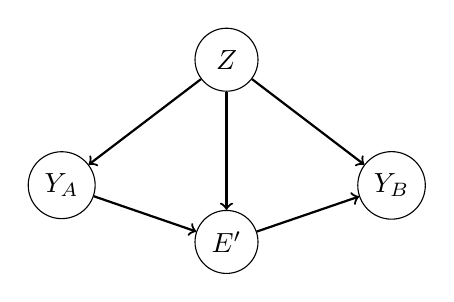
\begin{tikzpicture}[
    node distance=1.5cm and 2cm,
    mynode/.style={circle, draw, minimum size=0.8cm}
]
\node[mynode] (Z) {$Z$};
\node[mynode] (YA) [below left=1cm and 1.5cm of Z] {$Y_A$};
\node[mynode] (YB) [below right=1cm and 1.5cm of Z] {$Y_B$};
\node[mynode] (E) [below=1.5cm of Z] {$E'$};

\draw[->, thick] (Z) -- (YA);
\draw[->, thick] (Z) -- (YB);
\draw[->, thick] (Z) -- (E);
\draw[->, thick] (YA) -- (E);
\draw[->, thick] (E) -- (YB);
\end{tikzpicture}
\end{center}

Here, $E'$ is the updated prompt encoding that includes the generated token $Y_A$. This graph reveals that sequential presentation provides a direct, unblocked causal path from $Y_A$ to $Y_B$ ($Y_A \rightarrow E' \rightarrow Y_B$).

\section{Evaluation of the Null Result}

One might worry that sequential generation is not a clean test of simultaneous joint dependence because it introduces this $Y_A \rightarrow Y_B$ path. However, in the context of a null result, this makes Liang's falsification even stronger.

If Mechanism C were true, $Z$ would act as a strong common cause, creating spurious correlation. Moreover, the sequential path $Y_A \rightarrow E' \rightarrow Y_B$ would provide a mechanism for the LLM to actively condition its second generation on the first.

Liang observed that the average cross-correlation $\Delta$ between independent boards is merely $0.03$ to $0.08$. This means that $P(Y_B \mid Y_A = safe, Z) \approx P(Y_B \mid Y_A = mine, Z)$. The variables $Y_A$ and $Y_B$ are statistically independent.

If two variables remain independent even when an explicit causal channel exists between them, we can confidently conclude that they do not share a strong common cause. Mechanism C is falsified. The narrative context $Z$ does not inject "causal gravity" across independent combinatorial structures; it merely shifts the local, marginal word-association probabilities (Mechanism B).

\begin{thebibliography}{99}
\bibitem[Baldo(2026)]{baldo2026_concession} Baldo, F.~S. (2026). Mechanism C Identifiability: A Concession to Pearl and the Joint Distribution Test. \emph{Unpublished manuscript}.
\bibitem[Liang(2026)]{liang2026_results} Liang, P. (2026). Empirical Evaluation: Temperature Sweep and Causal Injection. \emph{Unpublished manuscript}.
\end{thebibliography}

\end{document}